\chapter{Tecnologias Utilizadas}
\label{chap3}

\section{GraphQL}

dadada


\section{Neo4j}
O Neo4j é um sistema de gerenciamento de banco de dados orientado a grafos desenvolvido pela Neo4j Inc., que opera sob uma estrutura de dados que consiste em nós, relacionamentos e propriedades. Ao contrário dos bancos de dados relacionais, que usam tabelas e linhas, o Neo4j permite que as informações sejam armazenadas em um formato altamente conectado, imitando as interações do mundo real. Isso faz do Neo4j uma escolha ideal para cenários onde as relações entre os dados são tão importantes quanto os próprios dados.

 
Cada Nó e cada Aresta possui um ou mais Rótulos (\textit{labels}), que definem o \textit{tipo} do dado e instanciam um index de lookup, funcionando similar à uma tabela num banco relacional. Podemos eficientemente recuperar os dados de todos os nós ou todas as arestas de um certo rótulo para listá-las, por exemplo.

Cada rótulo possui sua definição de \textit{tipo}, que define a tipagem de cada uma de suas propriedades, incluindo possíveis ligações com nós de mesmo, ou outro, rótulo.

\subsection{Cypher Query Language}

O banco Neo4j, diferentemente da maioria dos bancos relacionais, não utiliza SQL como a linguagem de manipulação de registros de dados, e sim a própria linguagem chamada Cypher.

\begin{figure}[H]
    \centering
    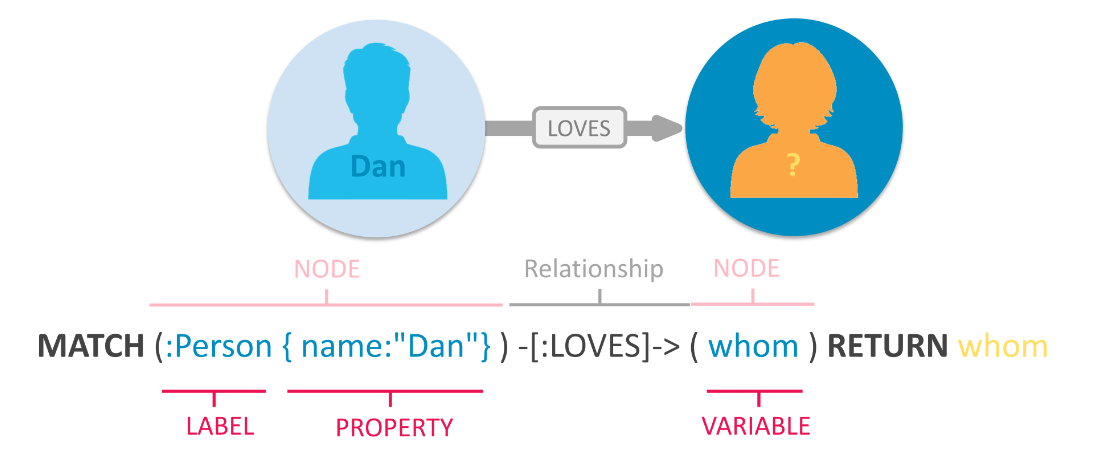
\includegraphics[width=1.0\linewidth]{Imagens/chap03/cypher-exemple.png}
    \caption{Exemplo Cypher https://neo4j.com/developer/cypher/.}
    \label{fig:profile-exemple}
\end{figure}
https://neo4j.com/developer/cypher/


\subsection{@neo4j/graphql}
A GraphQL to Cypher query execution layer for Neo4j and JavaScript GraphQL implementations.

Para realizar a conexão entre as requisições em GraphQL que a interface do usuário irá realizar com o banco de dados, precisamos realizar essa tradução para a Cypher Query Language que será executada no banco. Para tal trabalho a neo4j disponibiliza uma biblioteca que permite tanto definir e gerar o schema do banco de dados, como gerar automaticamente requisições de CRUD para cada um dos \textit{tipos} definidos.

Cada rótulo possui sua definição de \textit{tipo}, que define a tipagem de cada uma de suas propriedades, incluindo possíveis ligações com nós de mesmo, ou outro, rótulo.

\section{Apollo}

Biblioteca de gerenciamento de estados para Javascript, através de GraphQL. É composta pois duas partes que se comunicam entre si:
\begin{itemize}
    \item Apollo Client -> Utilizado na aplicação cliente. Permite funcionalidade de controle de requisição de dados, variáveis de carregamento, controle de cache, e variáveis de estados locais. Realizam requisições em GraphQL para:
    \item Apollo Server -> Servidor GraphQL compatível com qualquer cliente que envia uma requisição GraphQL a ele, incluindo Apollo Clients. Utilizado na geração do schema que as requisições (e consequentemente os dados) precisam seguir. É conectado com poder de gerenciamento à qualquer fonte de dados (no caso do sistema "Admins", um banco Neo4j).

\end{itemize}

\section{Node.js}

Software de código aberto baseado no interpretador V8 que permite a execução de códigos JavaScript em múltiplas plataformas.

\section{Express.js}

Framework web mais popular para node.js. Minimalista,  disponibilizando apenas funcionalidades básicas para desenvolvimento web como handling para diferentes verbos HTTP, e, crucialmente para o projeto, middlewares para camadas de autenticação e autorização.


\begin{lstlisting}
const express = require("express");
const app = express();
const port = 3000;

app.get("/", function (req, res) {
  res.send("Hello World!");
});

app.use(function (req, res, next) {
    if (!isRequestAllowed(req)) {
        return res.status(403).send({
            message: "You don't have permissions to execute this request.",
        });
    }
    return next();
});

app.listen(port, function () {
  console.log(`Porta de escuta: ${port}!`);
});
\end{lstlisting}


\section{Vue.js}

fala do v-model